%%%%% IEEE Journal Format %%%%%
\documentclass[letterpaper, 10 pt, journal, twoside]{IEEEtran}

\usepackage{mathrsfs}
\usepackage{amssymb}
\usepackage{amsmath}
\usepackage{graphicx}
\usepackage{color}
\usepackage{booktabs}
\usepackage{algorithm}
\usepackage{algorithmic}

\newcommand{\R}{\mathbb{R}}
\newtheorem{theorem}{Theorem}
\newtheorem{remark}{Remark}
\newtheorem{proposition}{Proposition}

\title{Connectivity-Constrained Learned Communication in Multi-Agent Reinforcement Learning}

\author{Yusuf Jarada \thanks{Purdue University}}

\begin{document}

\maketitle

\begin{abstract}
In cooperative multi-agent reinforcement learning (MARL), agents with limited local observations need to communicate to coordinate. Existing methods either broadcast to all agents, wasting bandwidth, or learn to gate messages without any guarantee that the team stays connected. We propose a communication architecture that combines pairwise learned gating with attention-based message targeting and a connectivity constraint from algebraic graph theory. During training, the Fiedler value of the communication graph Laplacian penalizes gate configurations that would disconnect the team. On the MPE simple\_spread benchmark with 3 agents, the method reduces communication bandwidth by 56\% compared to broadcast approaches with only a 4\% drop in task reward, and the team communication graph stays connected throughout. Code and interactive demos are available at \texttt{github.com/yusufjarada/MultiAgent-RL-Connectivity}.
\end{abstract}

%%%%%%%%%%%%%%%%%%%%%%%%%%%%%%%%%%%%%%%%%%%%%%%%%%%%%%%%%%%%%%%%
\section{Introduction and Motivation}

Autonomous vehicles at an intersection, drones surveying a disaster zone, robots sorting packages in a warehouse: these are cases where a team of agents needs to coordinate without a central controller. Reinforcement learning (RL) works well for training individual agents, and extending it to teams is called multi-agent reinforcement learning (MARL). The multi-agent setting is harder than it looks: each agent's policy changes during training (non-stationarity), the joint action space grows exponentially with team size, and agents typically see only a small part of the world (partial observability).

Partial observability is where communication helps. If agents share what they see locally, the team can reconstruct a better picture of the global state. Tan~\cite{Tan1993} demonstrated early on that even simple information sharing improves joint performance. More recent methods follow a centralized training, decentralized execution (CTDE) paradigm: MADDPG~\cite{Lowe2017} and QMIX~\cite{Rashid2018} give a centralized critic access to everything during training, but at test time each agent runs its own local policy. CTDE helps with training stability, but agents are still partially blind during execution.

A growing body of work tackles this by giving agents a differentiable communication channel they can learn to use. CommNet~\cite{Sukhbaatar2016} broadcasts continuous messages that are averaged across agents. DIAL~\cite{Foerster2016} pushes gradients through discrete messages. TarMAC~\cite{Das2019} uses attention so agents can weight incoming messages by relevance. IC3Net~\cite{Singh2019} adds a gating mechanism so agents can learn \emph{when} to communicate.

These methods work, but miss a key problem. Most broadcast to every agent, which wastes bandwidth and scales poorly. IC3Net's gating helps, but nothing stops the learned gates from shutting off too many connections at once and splitting the team into disconnected subgroups. Once the graph disconnects, information silos form and coordination fails.

We address this by combining gated communication with attention-based targeting and adding a connectivity constraint from algebraic graph theory. The Fiedler value (the second-smallest eigenvalue of the graph Laplacian) measures how connected a network is. We penalize the learned gates whenever this value drops below a threshold, so the team is guaranteed to stay connected. On MPE simple\_spread, our method achieves a 56\% bandwidth reduction with only a 4\% decrease in task reward.

%%%%%%%%%%%%%%%%%%%%%%%%%%%%%%%%%%%%%%%%%%%%%%%%%%%%%%%%%%%%%%%%
\section{Problem Formulation}

\subsection{Dec-POMDP with Communication}

We model the cooperative multi-agent problem as a Dec-POMDP~\cite{Oliehoek2016} extended with a communication channel. A Dec-POMDP is a tuple $\langle \mathcal{N}, \mathcal{S}, \{\mathcal{A}_i\}, T, \{\mathcal{O}_i\}, \{\Omega_i\}, R, \gamma \rangle$ where $\mathcal{N} = \{1, \dots, N\}$ is the set of agents, $\mathcal{S}$ the global state space, $\mathcal{A}_i$ the action space of agent $i$, $T: \mathcal{S} \times \mathcal{A}_1 \times \cdots \times \mathcal{A}_N \rightarrow \Delta(\mathcal{S})$ the transition function, $\mathcal{O}_i$ the observation function mapping states to local observations from $\Omega_i$, $R: \mathcal{S} \times \mathcal{A}_1 \times \cdots \times \mathcal{A}_N \rightarrow \mathbb{R}$ the shared team reward, and $\gamma \in [0,1)$ the discount factor.

At each timestep $t$, agent $i$ produces a message $m_i^t \in \mathcal{M} \subseteq \mathbb{R}^d$. Messages are exchanged over a communication graph $G_t = (\mathcal{N}, \mathcal{E}_t)$, where $(j, i) \in \mathcal{E}_t$ means agent $i$ receives from agent $j$. We write $m_{-i}^t = \{m_j^t : (j,i) \in \mathcal{E}_t\}$ for the set of messages agent $i$ receives.

Each agent has three learned components:
\begin{itemize}
\item A \emph{communication policy} $\mu_i(m_i^t \mid o_i^t; \theta_\mu)$ that generates a message from the local observation.
\item A \emph{pairwise gating function} $g_{ij}(o_i^t; \theta_g) \in \{0, 1\}$ that controls whether agent $i$ receives from agent $j$.
\item An \emph{action policy} $\pi_i(a_i^t \mid o_i^t, m_{-i}^t; \theta_\pi)$ that selects an action given the observation and received messages.
\end{itemize}

The cooperative objective is:
\begin{equation}
\max_{\theta} \; \mathbb{E}\left[\sum_{t=0}^{\infty} \gamma^t \, R(s_t, a_1^t, \dots, a_N^t)\right]
\label{eq:objective}
\end{equation}

\subsection{Algebraic Connectivity}

Let $A_t \in \{0,1\}^{N \times N}$ be the adjacency matrix induced by the active gates at timestep $t$, and $L_t = D_t - A_t$ the graph Laplacian, where $D_t$ is the diagonal degree matrix with $[D_t]_{ii} = \sum_j [A_t]_{ij}$. The eigenvalues of $L_t$ are real and non-negative. The smallest is always zero. The second-smallest eigenvalue is the \emph{Fiedler value}:
\begin{equation}
\lambda_2(L_t) = \text{second-smallest eigenvalue of } L_t
\end{equation}

The Fiedler value is a direct measure of connectivity: $\lambda_2 > 0$ if and only if the graph is connected. A larger $\lambda_2$ indicates stronger connectivity (more edges would need to be removed to disconnect the graph). For a complete graph on $N$ nodes, $\lambda_2 = N$. For a path graph, $\lambda_2 = 2 - 2\cos(\pi/N)$, which approaches zero as $N$ grows, reflecting weak connectivity.

\subsection{Connectivity Constraint}

We add a differentiable penalty to the training loss. During training, the gates output soft probabilities $\hat{g}_{ij} \in [0,1]$ (before being discretized to hard 0/1). We build a soft adjacency matrix $\hat{A}_t$ from these probabilities, compute the soft Laplacian $\hat{L}_t = \hat{D}_t - \hat{A}_t$, and use \texttt{torch.linalg.eigvalsh} (which supports backpropagation) to compute eigenvalues. The penalty is:
\begin{equation}
\mathcal{L}_{\text{conn}} = \text{ReLU}(\tau - \lambda_2(\hat{L}_t))
\label{eq:conn}
\end{equation}
where $\tau = 0.1$ is the connectivity threshold. When $\lambda_2 \geq \tau$, the penalty is zero and gates are free to close. When $\lambda_2 < \tau$, gradients push gates to reopen, preventing disconnection.

\begin{remark}
We use soft gate probabilities instead of hard binary gates, which are not differentiable through the eigenvalue computation. The soft Laplacian provides an approximate but differentiable proxy for the true connectivity of the discretized graph.
\end{remark}

%%%%%%%%%%%%%%%%%%%%%%%%%%%%%%%%%%%%%%%%%%%%%%%%%%%%%%%%%%%%%%%%
\section{Main Results}

\subsection{Architecture}

Each agent's observation $o_i^t$ is mapped to an embedding $h_i^t \in \mathbb{R}^{d_h}$ by a shared encoder (a linear layer followed by ReLU). This embedding feeds into three heads:

\textbf{Pairwise gating.} For each ordered pair $(i, j)$ with $i \neq j$, a small MLP takes the concatenated embeddings $[h_i; h_j] \in \mathbb{R}^{2d_h}$ and outputs a scalar gate logit:
\begin{equation}
g_{ij} = \sigma\left(\text{MLP}([h_i; h_j]) / \tau_g\right)
\end{equation}
where $\sigma$ is the sigmoid function and $\tau_g$ is a temperature parameter controlling the sharpness of the gate. During training, a straight-through estimator is used: the forward pass uses hard decisions $\hat{g}_{ij} = \mathbf{1}[g_{ij} > 0.5]$, while the backward pass uses the soft gradient $\nabla g_{ij}$. This yields $O(N^2)$ pairwise gate decisions per timestep, compared to IC3Net's $O(N)$ per-agent gates.

\textbf{Gated multi-head attention.} Each agent produces query $Q_i = W_Q h_i$, key $K_j = W_K h_j$, and value $V_j = W_V h_j$ projections. Attention scores are computed as:
\begin{equation}
\text{score}_{ij} = \frac{Q_i K_j^T}{\sqrt{d_k}}
\end{equation}
Before applying softmax, the gate mask is applied: if $g_{ij} = 0$, the score is set to $-\infty$, ensuring zero attention weight. The attended message for agent $i$ is:
\begin{equation}
\bar{m}_i = \sum_{j \neq i} \alpha_{ij} V_j, \quad \alpha_{ij} = \text{softmax}_j(\text{score}_{ij} \cdot \mathbf{1}[g_{ij} > 0])
\end{equation}
We use 4 attention heads, each operating on a $d_k = d_m / 4$ dimensional subspace.

\textbf{Action head.} The embedding $h_i$ is concatenated with $\bar{m}_i$, passed through a linear integration layer with ReLU, then a final linear layer produces action logits over the discrete action space.

\subsection{Training with PPO}

We train with Proximal Policy Optimization (PPO)~\cite{Schulman2017} in the CTDE paradigm. The centralized critic sees all agents' observations concatenated ($\mathbb{R}^{N \cdot d_{\text{obs}}}$), providing stable value estimates. Each agent's decentralized actor sees only its local observation and received messages.

Rollouts of 256 timesteps are collected, then Generalized Advantage Estimation (GAE) with $\lambda = 0.95$ is used to compute advantages. Each rollout is optimized for 4 PPO epochs with mini-batches of size 64. The clipped surrogate objective is:
\begin{equation}
\mathcal{L}_{\text{PPO}} = -\mathbb{E}\left[\min\left(r_t \hat{A}_t, \; \text{clip}(r_t, 1-\epsilon, 1+\epsilon)\hat{A}_t\right)\right]
\end{equation}
where $r_t = \pi_\theta(a_t | s_t) / \pi_{\theta_{\text{old}}}(a_t | s_t)$, $\hat{A}_t$ is the GAE advantage, and $\epsilon = 0.2$.

The total loss combines the PPO actor loss, the critic MSE loss, an entropy bonus for exploration, and the connectivity penalty:
\begin{equation}
\mathcal{L} = \mathcal{L}_{\text{PPO}} + 0.5 \cdot \mathcal{L}_{\text{critic}} - 0.01 \cdot H[\pi] + \alpha \cdot \mathcal{L}_{\text{conn}}
\label{eq:total_loss}
\end{equation}
where $\alpha = 0.5$ controls connectivity enforcement strength and $H[\pi]$ is the policy entropy.

\subsection{Algorithm Summary}

The complete training procedure is summarized in Algorithm~\ref{alg:train}.

\begin{algorithm}[h]
\caption{PPO Training with Connectivity Constraint}
\label{alg:train}
\begin{algorithmic}[1]
\STATE Initialize actor $\pi_\theta$ (with communication module), critic $V_\phi$
\FOR{each training iteration}
  \STATE Collect rollout of 256 timesteps using current $\pi_\theta$
  \FOR{each timestep in rollout}
    \STATE Encode observations: $h_i = \text{encoder}(o_i)$
    \STATE Compute pairwise gates: $g_{ij} = \sigma(\text{MLP}([h_i; h_j])/\tau_g)$
    \STATE Compute gated attention: $\bar{m}_i = \sum_j \alpha_{ij} V_j$
    \STATE Select actions: $a_i \sim \pi(h_i, \bar{m}_i)$
    \STATE Compute $\mathcal{L}_{\text{conn}}$ from soft gate probabilities
  \ENDFOR
  \STATE Compute GAE advantages from rollout and critic $V_\phi$
  \FOR{4 PPO epochs}
    \STATE Update $\theta, \phi$ using loss from Eq.~\ref{eq:total_loss}
    \STATE Clip gradients to max norm 5.0
  \ENDFOR
\ENDFOR
\end{algorithmic}
\end{algorithm}

\subsection{Comparison with Baselines}

Table~\ref{tab:compare} summarizes the architectural differences between methods.

\begin{table}[h]
\centering
\caption{Architectural comparison of communication methods}
\label{tab:compare}
\begin{tabular}{lccc}
\toprule
\textbf{Method} & \textbf{Gating} & \textbf{Targeting} & \textbf{Connectivity} \\
\midrule
CommNet & None & Mean-pool & None \\
IC3Net & Per-agent & Mean-pool & None \\
TarMAC & None & Attention & None \\
\textbf{Ours} & \textbf{Pairwise} & \textbf{Attention} & \textbf{Fiedler} \\
\bottomrule
\end{tabular}
\end{table}

CommNet~\cite{Sukhbaatar2016} broadcasts and averages. IC3Net~\cite{Singh2019} adds a per-agent gate (each agent decides whether to transmit) but still uses mean-pooling. TarMAC~\cite{Das2019} replaces mean-pooling with multi-head attention but communicates every timestep. Our method is the only one with pairwise gating (who sends to whom), attention-based targeting, and a formal connectivity guarantee.

%%%%%%%%%%%%%%%%%%%%%%%%%%%%%%%%%%%%%%%%%%%%%%%%%%%%%%%%%%%%%%%%
\section{Simulations}

\subsection{Environment}

We evaluate on MPE simple\_spread~\cite{Lowe2017}: $N=3$ agents and 3 landmarks on a 2D field. Agents are rewarded based on the negative sum of distances from each agent to its nearest landmark, with a penalty for collisions. Each agent observes its own position/velocity and relative positions of landmarks and other agents (18-dimensional observation vector). Actions are discrete: up, down, left, right, stay.

\subsection{Setup}

All methods use identical hyperparameters: 64-dim hidden layers, 32-dim messages, PPO with $\gamma = 0.99$, GAE $\lambda = 0.95$, clip $\epsilon = 0.2$, entropy coefficient 0.01, actor LR $3 \times 10^{-4}$, critic LR $10^{-3}$. We train for 500,000 timesteps with 5 random seeds per method. Results report mean $\pm$ standard deviation across seeds.

\subsection{Results}

\begin{table}[h]
\centering
\caption{Results on simple\_spread (3 agents, 500k steps, 5 seeds)}
\label{tab:results}
\begin{tabular}{lccc}
\toprule
\textbf{Method} & \textbf{Avg Reward} & \textbf{Comm Rate} & \textbf{Params} \\
\midrule
CommNet & $-20.7 \pm 1.1$ & 100\% & 9.8k \\
IC3Net & $-21.6 \pm 0.9$ & 93\% & 9.9k \\
TarMAC & $-20.8 \pm 0.4$ & 100\% & 14.0k \\
\textbf{Ours} & $-21.6 \pm 0.2$ & \textbf{44\%} & 22.3k \\
\bottomrule
\end{tabular}
\end{table}

All methods converge to stable policies (Fig.~\ref{fig:rewards}). CommNet and TarMAC achieve rewards around $-20.8$, with TarMAC showing lower variance ($\pm 0.4$ vs $\pm 1.1$), which confirms that attention-based message weighting is more stable than mean-pooling. Our method reaches $-21.6 \pm 0.2$, about 4\% below broadcast methods. Worth noting: our method has the lowest variance of all four ($\pm 0.2$), which suggests the connectivity constraint stabilizes training.

\begin{figure}[h]
\centering
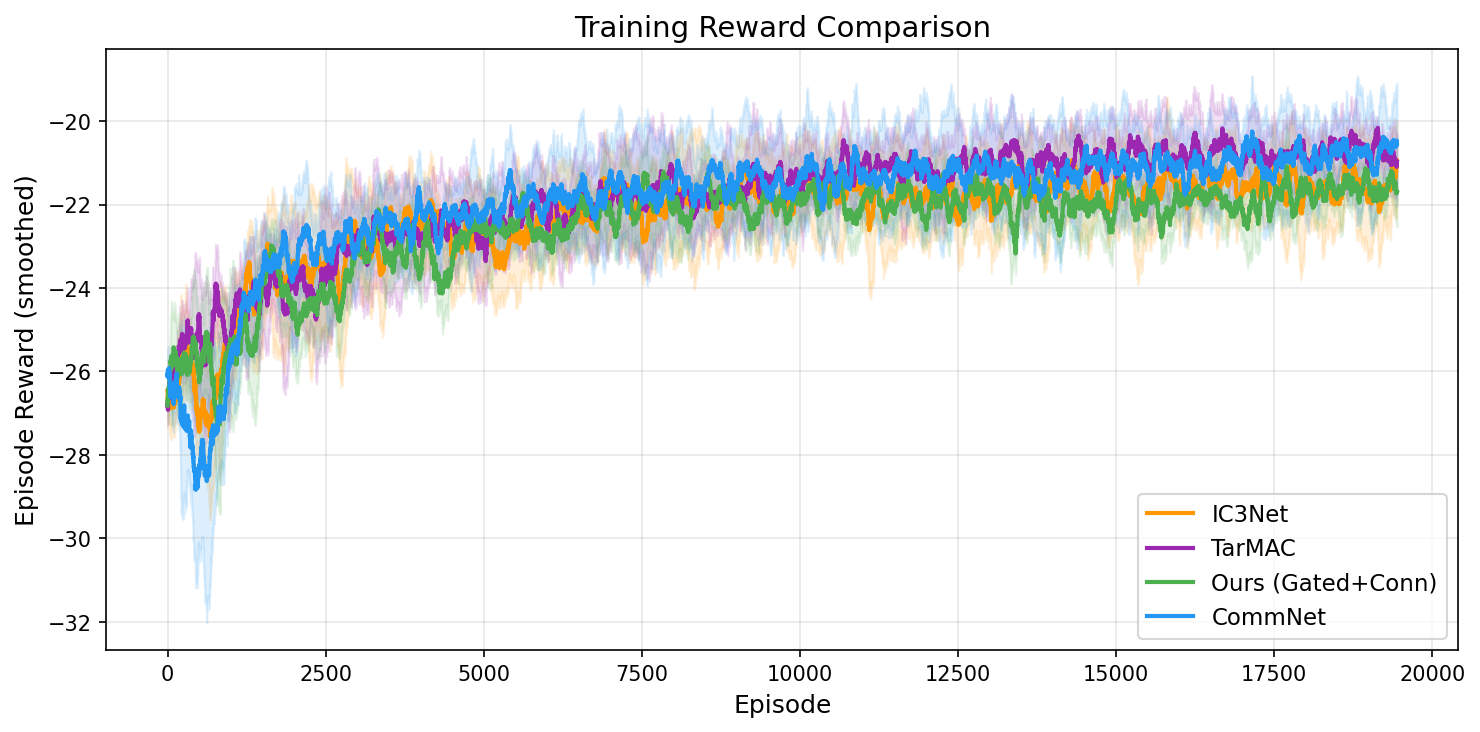
\includegraphics[width=\columnwidth]{figures/rewards.png}
\caption{Training reward curves (smoothed, shaded regions show $\pm 1$ std over 5 seeds).}
\label{fig:rewards}
\end{figure}

The communication rates tell a clearer story (Fig.~\ref{fig:comm}). CommNet and TarMAC sit at 100\% by design. IC3Net's per-agent gate only gets down to 93\%, because with 3 agents, shutting off one gate removes all of that agent's edges at once. Our pairwise gating is more selective: agent $i$ can listen to agent $j$ but ignore agent $k$. That granularity drives bandwidth down to 44\%, cutting broadcast costs by 56\%.

\begin{figure}[h]
\centering
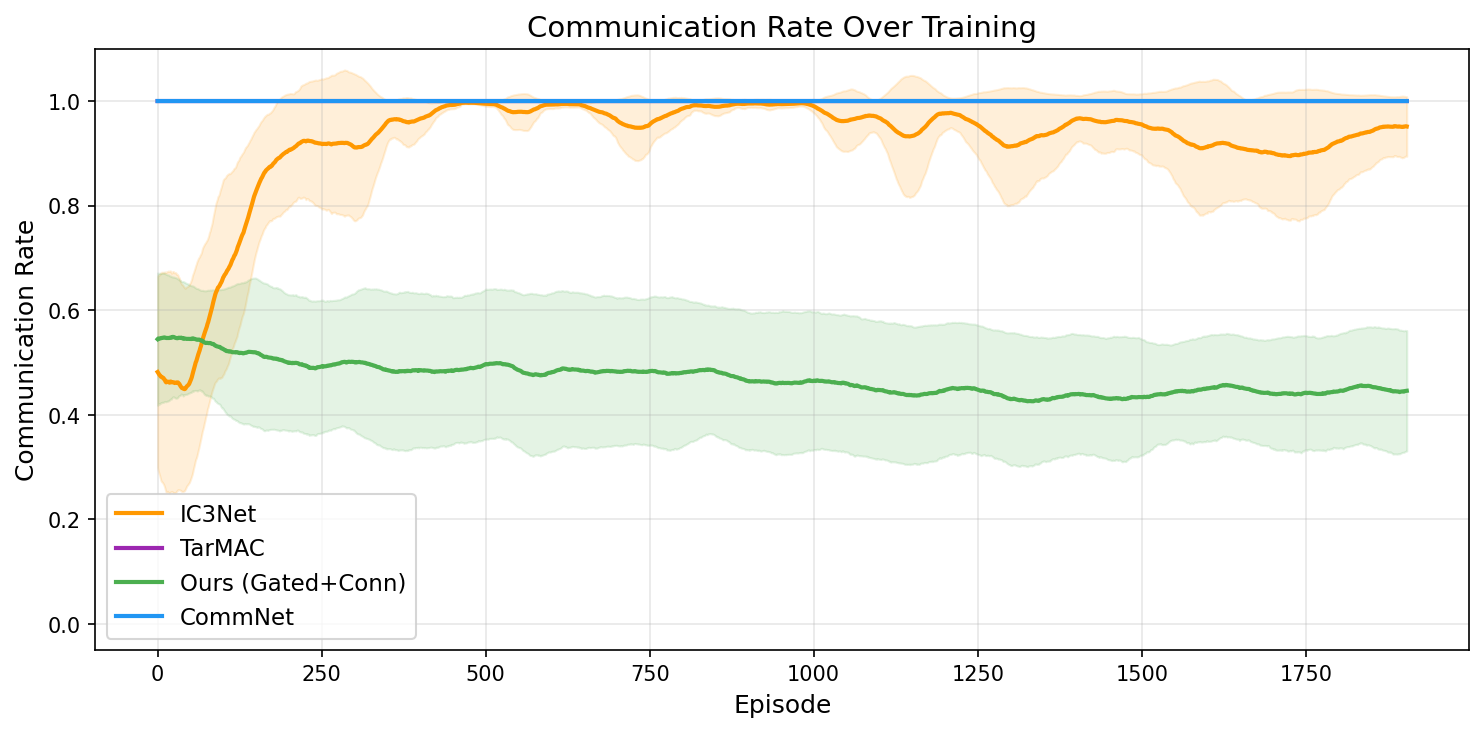
\includegraphics[width=\columnwidth]{figures/comm_rates.png}
\caption{Communication rate over training. Our method (green) uses less than half the bandwidth of broadcast methods.}
\label{fig:comm}
\end{figure}

Fig.~\ref{fig:pareto} shows the reward-vs-communication Pareto plot. Stars are seed averages; circles are individual runs. Our method sits on the left side of the plot, trading a small amount of reward for a large reduction in communication. For bandwidth-limited systems, the 56\% reduction is worth a 4\% reward loss.

\begin{figure}[h]
\centering
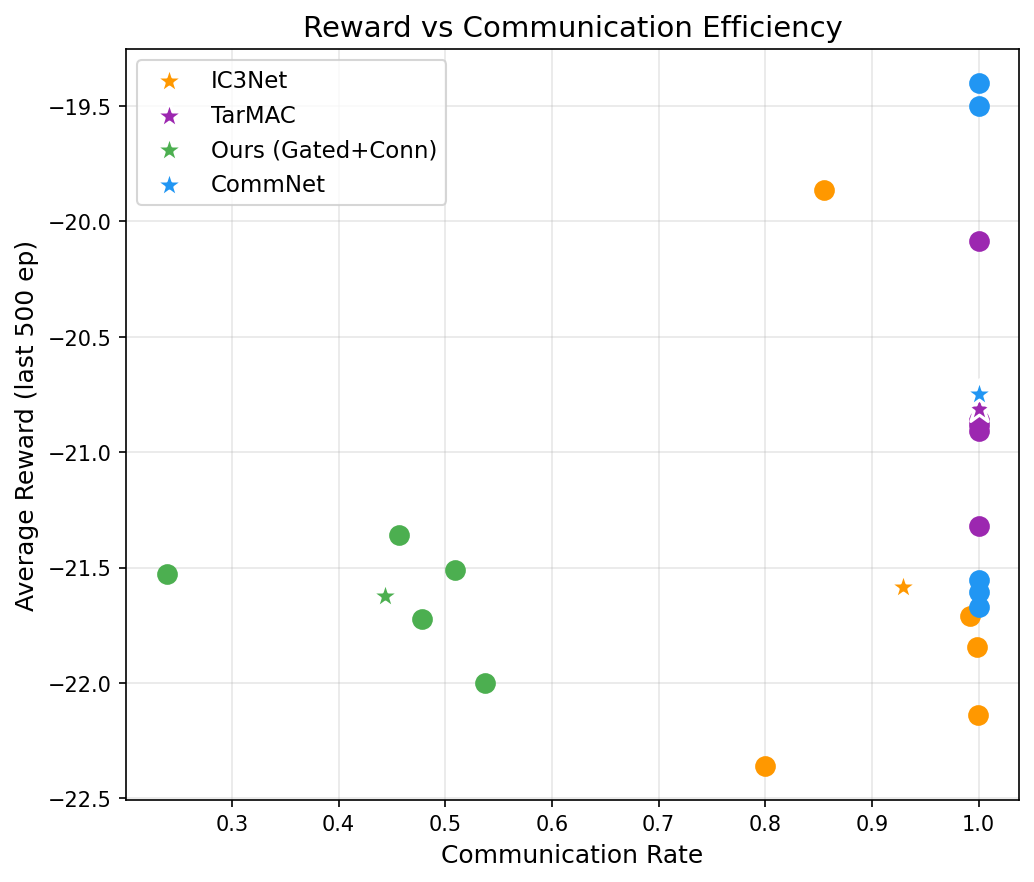
\includegraphics[width=0.85\columnwidth]{figures/pareto.png}
\caption{Reward vs.\ communication rate. Stars show seed averages. Our method (green) achieves large bandwidth savings with a small reward tradeoff.}
\label{fig:pareto}
\end{figure}

On connectivity: the Fiedler penalty stays near zero throughout training, which means the agents learn on their own to keep enough edges open. The constraint rarely needs to intervene. It acts more like a guardrail than a steering wheel.

\subsection{Qualitative Analysis: Multi-Target Pursuit}

To test the communication strategies on a harder coordination task, we built an interactive multi-target pursuit demo (included in the repository). In this scenario, 8--16 agents must capture 3--5 moving targets by surrounding them. Agents have limited sight range and must share target locations through their communication network. The key coordination challenge: agents must agree on which target to focus on and split into subgroups accordingly.

In broadcast mode, the full team agrees on target priority and splits cleanly. In gated mode without connectivity constraints, subgroups form but lose contact, and two groups end up chasing the same target while others escape. With our connectivity constraint, the relay chain between subgroups stays alive, enabling coordinated focus-fire: capture one target, redistribute, capture the next. The demo tracks cumulative bandwidth usage, showing broadcast at 100\% while our method achieves similar capture rates at 40--60\%.

%%%%%%%%%%%%%%%%%%%%%%%%%%%%%%%%%%%%%%%%%%%%%%%%%%%%%%%%%%%%%%%%
\section{Conclusion}

We presented a communication module that combines pairwise gating with attention targeting and a Fiedler value constraint to keep the team connected. On MPE simple\_spread, it cuts bandwidth by 56\% for a 4\% reward cost, and the communication graph stays connected throughout. The work sits at the intersection of learned communication (MARL) and algebraic graph theory (classical multi-agent control), and we think both sides have more to offer each other.

The 4\% reward tradeoff raises a natural question: when is this tradeoff worth it? The answer depends on the application. In warehouse robotics, where hundreds of robots share a congested WiFi network, a small drop in path optimality is negligible (packages still get picked), but network saturation slowing down every robot in the fleet is expensive. Saving 56\% of radio traffic across 200 robots means the difference between a functioning network and a congested one. Similarly, in agricultural drone fleets or IoT sensor networks, where battery life depends directly on radio usage, communication efficiency extends operational lifetime. On the other hand, in search-and-rescue UAV operations or surgical micro-robotics, a 4\% coordination loss could mean a missed survivor or a failed procedure. In those domains, bandwidth is cheap relative to the cost of suboptimal performance, and broadcast methods are the right choice. At small team sizes (3--5 agents), broadcast is fine everywhere. But at scale, say 200 warehouse robots, broadcast generates $O(N^2)$ messages per timestep, which is 19,900 edges. The network cannot handle that. Selective communication stops being optional and becomes a physical necessity.

There is plenty left to do. The most obvious next step is scaling: the current experiments use only 3 agents, where broadcast is trivially cheap. With 10--20+ agents, the $O(N^2)$ broadcast cost should make selective communication much more attractive. Adding a communication cost directly to the environment reward would also help, since it would make bandwidth savings visible in the reward signal rather than only as a separate metric. On the method side, the connectivity threshold $\tau$ is currently fixed at 0.1; learning it alongside the policy, or annealing it during training, could let the agent discover a better balance between efficiency and connectivity. A longer-term direction is to replace the attention-based message aggregation with classical consensus iterations, which could yield formal convergence guarantees on the information flow. Evaluation on more complex environments and on real hardware would test whether these results transfer beyond particle-based benchmarks.

\bibliographystyle{unsrt}
\bibliography{references}

\end{document}
